\section{React}

\begin{itemize}
	\item für die Implementation von grossen Applikationen
	\item ist eine JavaScript Bibliothek für den View einer SPA
	\item reduziert die Applikationsentwicklung auf reines JavaScript
	\item basiert auf JavaScript-Komponenten
	\item führt einen Virtuellen DOM
	\item minimiert dadurch die Manipulationen des DOMs im Browser
	\item nutzt keine HTML-Templates
	\item führt JSX als Erweiterung von JavaScript ein
	\item nutzt Properties um read-only Eigenschaften zu definieren
	\item nutzt State um den Zustand einer Komponenten zu beschreiben
	\item nutzt die Methode render() der Komponente, um die Komponente zu zeichnen
	\item ruft bei jeder Änderung des State die Methode render() automatisch auf
\end{itemize}

\subsection{Komponenten}
Komponenten erlauben eine Benutzeroberfläche in unabhängige, wiederverwendbare Teile aufzubrechen und jeden als isoliert zu betrachten.

\textbf{Nutzen:} Wird an einer Komponente etwas geändert, müssen die übrigen Komponenten nicht getestet werden, da diese nicht von den Änderungen betroffen sein können.

Reacts zentraler und einziger Baustein sind Komponenten.

Eine React Komponente muss immer eine render() Methode haben.

\subsection{Properties einer Komponente}

Properties werden von aussen an die Komponente bergeben (analog Input Parameter einer Methode). Innerhalb der Komponente sind Properties nicht veränderbar.

\subsection{State einer Komponente}

Eine React-Komponente kann einen Zustand (State) besitzen, der sich zur Laufzeit ändert. Der State beschreibt die veränderlichen Daten der Komponente. Wichtig: Nur die Komponente selber kann seinen State mit setState(...) verändern. Eine Änderung am State löst automatisch einen Call auf die Methode render() aus. Die Komponente und ihre Kinder werden neu gezeichnet.

\subsection{Lifecylce einer Komponente}
Die Methode "componentDidMount()" wird con React aufgerufen, sobald die Komponente an den virtuellen DOM-Tree eingebunden ist.

Die Methode "componentWillUnmount()" wird aufgerufen kurz bevor die Komponente aus dem DOM-Tree entfern und gelöscht wird.

\subsection{Functional Component}
React Component\\
• Komponente ist eine Klasse\\
• Stateful\\
\\
React Functional Component\\
• Komponente ist eine Funktion\\
• Stateless\\
• Kein this Keyword\\
• Weniger Code\\
• Destructuring\\

\begin{minted}{JavaScript}
class App extends Component {

    constructor(props) {
        super(props);

        this.state = {
            counter: 0
        }
    }

    componentDidMount() {
        this.timer = setInterval(this.increment, 1000);
    }

    componentWillUnmount() {
        clearInterval(this.timer);
    }

    increment = () => {
        this.setState({counter: this.state.counter + 1});
    }
    reset = () => {
        this.setState({counter: 0});
    }

    render() {
        return (
            <div className="container">
                <div>
                    <Jumbotron>
                        <h1>{this.state.counter}</h1>
                    </Jumbotron>
                </div>
                <div>
                    <Button onClick={this.reset}>RE-FRÄSCH</Button>
                </div>
            </div>

        )
    }

}
\end{minted}

\section{Virtueller DOM}
Die Manipulation des Document Object Models (DOM) im Browser ist teuer und deshalb langsam.
Jede Änderung an dieser Baumstruktur quittiert der Browser mit teurer Neuberechnung seiner Geometrie.
Je mehr geändert wird, desto länger dauert es. Je weniger man den DOM des Browsers verändert, desto schneller ist die Applikation.

JavaScript selber ist performant:
Viele JavaScript-Frameworks suchen einen Kompromiss mittels Verwendung von altbewährten Entwurfsmustern, um die Komplexität zwischen Einfachheit und Performance zu bändigen. (Two-way binding, dirty-checking, etc.)
React versucht es mit einem extremen Ansatz, der in erster Linie die Einfachheit und nicht die Performanz in den Fokus stellt. React rendert bei jedem Update einfach alles neu!

Virtueller DOM:
Mit React Komponenten und JSX arbeitet man nicht direkt mit dem DOM des Browsers, sondern mit normalen JavaScript Objekten (--> Virtueller DOM), die schnell gelesen und bearbeitet werden können, ohne dass damit tatsächliche Änderungen am DOM ausgelöst werden.
Bei jeder Änderung der Daten erstellt React einen neuen virtuellen DOM.
Ein stark optimierter und heuristischer Algorithmus vergleicht diesen neuen Baum mit den vorherigen und errechnet eine Liste von minimalen Änderungen am richtigen DOM aus.
Diese werden gesammelt und nicht direkt, sondern im Batch (=Stapel) an den Browser weitergeleitet.

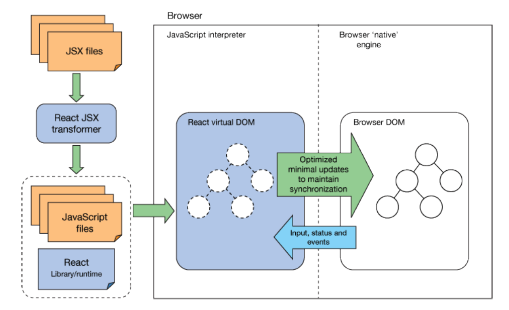
\includegraphics[width=\columnwidth]{images/dom}

Reconciliation beschreibt den Mechanismus, der
die Zustandsänderungen in einer React-Komponente beobachtet.
einen aktualisierten Zustand auf den Bildschirm schreibt.

Fragen zum virtuellen DOM
\begin{itemize}
	\item  Wann wird eine Reconciliation-Phase ausgelöst?
	\item  Welche Änderungen im Component Tree sind "teuer" und welche "billig"?
	\item  Was ist die Funktion eines "key" in einer Liste?
	\item Welche Schritte in der Reconciliation-Phase werden bei der React-App aus Übung 6 konkret ausgeführt?
\end{itemize}



\section{Hooks}

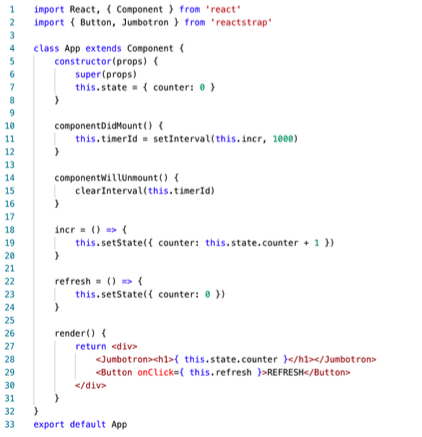
\includegraphics[width=0.7\columnwidth]{images/withouthooks}

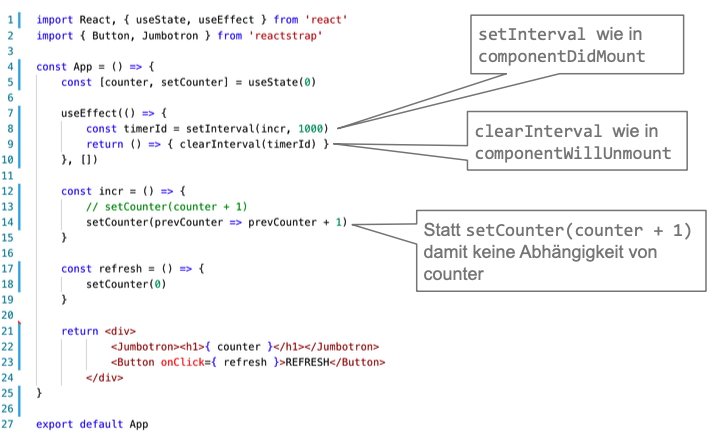
\includegraphics[width=0.8\columnwidth]{images/withhooks}

\subsection{Hooks Regeln}
\begin{itemize}
	\item Hooks dürfen nur vom Top-Level der Funktionalen Komponente aufgerufen werden.
	\item Die Reihenfolge von Hook-Aufrufen muss immer gleich bleiben.
\end{itemize}